\section{Sauvetage du Pelican}

Voici un premier scénario pour la campagne \textbf{Dos au Muur}. 

\subsection{La rencontre}
Nos héros ne se connaissent pas encore. Ils ont répondu à un contrat proposé par \emph{Industrial Automaton} pour une mission de récupération.

\begin{paperbox}{Notes sur les personnages}
	Je n’aime pas brider les joueurs sur leur choix de concept de personnage. Mais des fois l’imagination des joueurs dépasse légèrement le cadre de nos scénarios. Alors voici quelques exemples de concepts et comment il est possible de les intégrer :
	\begin{rebelist}
		\item Des \textbf{mercenaires} et chasseurs de primes, qui du coup s’intègrent très bien dans le scénario
		\item Un \textbf{mécano} touche à tout, qui était envoyé par IA pour sa connaissance du vaisseau ou du modèle R4
		\item Un \textbf{noble}, qui en tant qu’investisseur voulait savoir ou passe son argent (et IA qui voulant s’en débarrasser a accepté avec plaisir)
	\end{rebelist}
\end{paperbox}

Ils ont rendez-vous sur l’avant-poste commercial de l’anneau de Kafrene au Starlord Café. \'A leur arrivée, ils sont conviés dans une arrière salle ou les attend \nameref{vyna-anen} un Sluissi, le représentant de IA. En plus du groupe de nos héros, deux autres personnes ont répondu au contrat, un Abyssin et un Rodien.

\begin{quotebox}
	Messieurs bonjour, je représente Indrustrial Automaton.
	Comme vous avez peu le voir sur le contrat auquel vous avez répondu, nous cherchons à rassembler une équipe pour récupérer l’un de nos prototypes de droïde Type R perdu sur un Croiseur dont nous n’avons plus de nouvelle.
	Le \textbf{Pelican IA-1701} n’a plus donné signe de vie depuis 10h et 33mn maintenant. Il avait à son bord le seul prototype de notre dernier Type R. Il est vital pour nous de récupérer ce prototype intact.

	Si vous acceptez la mission, une navette droïde vous conduira directement à la dernière position connue du Pelican. Cette mission doit resté confidentielle, nous ne tenons pas à ce que le public sache qu’Industrial Automaton perde ses vaisseaux !
	En cas de succès la somme convenue sera virée directement sur vos comptes respectifs. Dans le cas contraire vous serez mort ou en passe de l’être.

	Y a-t’il des questions ?

	\ldots

	Bien, la navette décollera de l’astroport, quai N°5 dans une heure, elle n’attendra personne.
\end{quotebox}

Voilà qui donne le ton et la direction du scénario. Les héros disposent donc d’une heure, s’ils le souhaitent pour faire quelques emplettes puis direction la navette. Si des joueurs demandent à prendre leur propre vaisseau, cela est impossible, l'emplacement du vaisseau doit rester confidentiel.

\subsection{Pelican Bay}
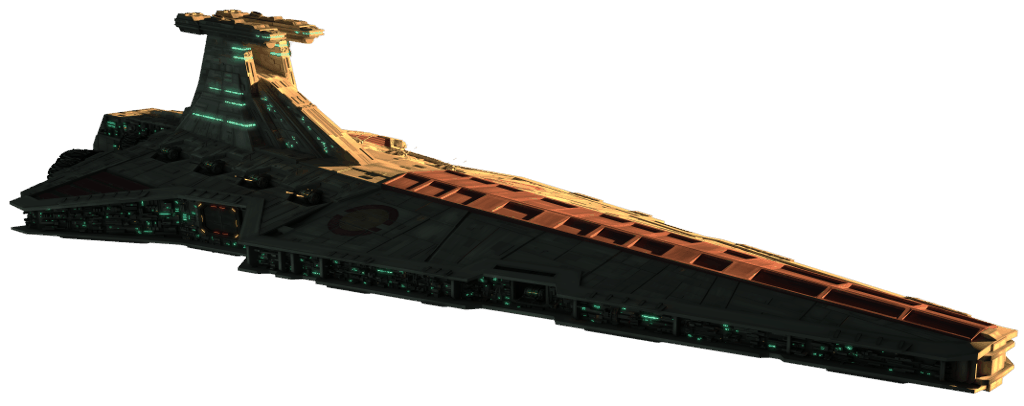
\includegraphics[width=\linewidth]{_img/dos-au-muur/venator.png}
\'A la sortie d’hyperespace, les héros trouvent croiseur de classe Venator en bon état mais à la dérive. La navette tente une procédure d’appontage mais le système de guidage ne semble pas fonctionner, le droïde aux commandes de la navette ne cesse de répéter :
\begin{quotebox}
	Erreur trop bas trop bas !\\
	Erreur trop bas trop bas !\\
	Erreur trop bas trop bas !\\
	Erreur trop bas trop bas !\\
	Erreur trop bas trop bas !\ldots
\end{quotebox}

Et la navette s’échoue lamentablement dans le hangar. Comme de par hasard, et pour bien appuyer sur la gravité de la situation, l’Abyssin et le Rodien sont mort pendant le crash et le droïde pilote est dans un sale état. Il ne pourra donner aucune information.

Une fois à bord du Pelican, une alarme est en cours et une voie pré-enregistrée se fait entendre à intervalles réguliers :

\begin{quotebox}
	Alerte trajectoire, le vaisseau se dirige actuellement vers une étoile, point de non-retour dans 2h53mn ! 
	Voyez modifier la trajectoire du vaisseau !\\ 
	\ldots
\end{quotebox}

\'A l’intérieur du vaisseau c’est la désolation, des cadavres partout, du sang sur les murs, des traces de griffures sur les murs. L’éclairage est partiellement en panne les néons scintillent, des débris entravent la marche des héros. Leur champ de vision est réduit à cause des conditions à bord. Malgré tout ça, les systèmes de survie et la gravité artificielle fonctionnent.\\

Le bruit du crash de la navette a attiré la population locale, à savoir les Rakghouls~\ref{sec:rakghoul} (p. \pageref{sec:rakghoul}). Lancer 1d4 pour savoir combien se pointent. Si vous n’avez que 2 ou trois héros sous la main, ajustez avec 1d4-1.

\noindent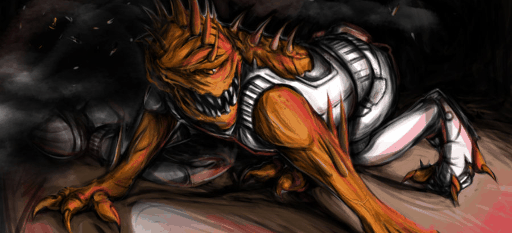
\includegraphics[width=\linewidth]{_img/dos-au-muur/rakghoul.png}

Le but des héros devrait maintenant être double, trouver le fameux prototype mais aussi trouver un moyen de sauver leur peau. 

\subsection{Exploration}
\emph{Numérotez les pièces de votre vaisseau et lancez un dé pour savoir dans quelle pièce se trouve le droïde.}\\

Une fois la première vague de Rakghouls balayé, nos héros se retrouvent dans le hangar, la porte de se dernier est ouverte.

Un jet de Recherche (-2 pour l’obscurité) réussi permet de trouver un kit de survie avec un Medipac, une lampe torche et des rations de survie.

Pas loin de la porte du hangar se trouve un terminal dont l’écran clignote en rouge au rythme de l’alarme. Les héros peuvent tenter des jets de Piratage pour les actions suivantes :
\begin{rebelist}
	\item Stopper l’alarme. 
	\item Obtenir un plan du vaisseau. En cas de succès, le plan s’affiche mais le terminal rend l’âme au bout de quelques secondes et le plan s’efface. En cas de relance le plan reste affiché et le terminal est utilisable.
	\item Obtenir l’inventaire des navettes présente dans les hangars du vaisseau. Un succès leur apprend qu’il y en a une dans le hangar du niveau inférieur. Une Relance leur apprend que la navette est dans le hangar 4-2.
\end{rebelist}
Dans tous les cas, un échec critique fait disjoncter le terminal définitivement.

Les héros avancent donc dans les couloirs du Pelican à la recherche du droïde et d’un moyen de dévier le vaisseau. Faites faire un jet de Discrétion de temps à autre. En cas d’échec, 2 Rakghouls se pointent (plus si vous voyez que vos héros s’en tire trop facilement).

Au fur et mesure que les aventuriers avancent, utilisez les tuiles pour découvrir la carte du vaisseau.

\subsubsection{Le Droïde}
Quand les héros arrivent dans la salle où se trouve le droïde (\nameref{sec:r4-3d}), ce dernier les menace avec un arc électrique, rien de bien méchant mais les héros doivent le rassurer et Négocier (jet de Persuasion) avec le droïde ou le Pirater (jet de Piratage opposé à l’Intellect). Dans les deux cas, avec un succès, le droïde les aide, leur montre le journal de bord. Avec une Relance, le droïde devient un acolyte du héros qui a fait l’action. En cas d’échec le droïde refuse de les aider il se désactive. En cas d’échec critique, le droïde s’en prend à eux.

Si le droïde se désactive, un héros peut tenter de lui retirer la mémoire pour récupérer les infos avec un jet de Réparation. 

\subsubsection{Les Quartiers}
Il s’agit des quartiers de l’équipage. Pas grand-chose à y trouver, des vêtements, des effets personnels. On y trouve des terminaux qui peuvent être Piraté pour le plan du vaisseau ou pour d’autres informations. Avec un succès, ils se connectent et ont accès au contenu du PC. La carte s’ils la cherchent, sinon rien de fou, des photos, des vidéos et des films X.

\subsubsection{Les Laboratoires}
La porte du premier labo que les héros visitent est verrouillé. un jet de Piratage la déverrouille. Si le droïde est avec eux et les aide, il peut ouvrir toutes les portes. Les aventuriers trouvent dans ce labo le corps du rakghoul et un terminal. Un Piratage (malus -2, c’est un terminal sécurisé) leur donne les informations sur l’autopsie (cf. Le \nameref{sec:pelican-jdb} p. \pageref{sec:pelican-jdb}), pas plus sur les circonstances.

Dans les autres labos, un jet de recherche donne un Medipac supplémentaire.

\subsubsection{L’Armurerie}
Dans cette pièce se trouvent des cellules énergétiques pour les armes et des armes mais enfermées dans des casiers. Un coup de blaster ouvre les casiers. On trouve alors 
\begin{rebelist}
	\item 5x Blaster semi-automatique \emph{(2d8 (3))}
	\item 1x Lance-Grenades \emph{(2d10 (1))}
	\item 5x Grenade \emph{(3d6)}
\end{rebelist}

\subsubsection{La Passerelle}
La pièce est verrouillée et ne peut être ouverte avec un Piratage. Seul le droïde peut l’ouvrir. Si le droïde disparaît ou s’éteint, la salle s’ouvre. Les héros en entrant dans la pièce trouvent le corps décomposé du commandant. En recherchant dans les poches du commandant, ils trouvent un document marqué "Protocole d’Urgence" expliquant la marche à suivre en cas de problème (cf. Le \nameref{sec:pelican-jdb} p. \pageref{sec:pelican-jdb}). Le papier contient aussi les codes d’accès au terminal.

Les héros peuvent donc accéder au \nameref{sec:pelican-jdb} avec toutes les infos. Si cela n’est déjà connu, ils savent qu’un vaisseau en état les attend dans le hangar 4-2 et il est possible d’en ouvrir la porte depuis ce terminal. S’ils sont malins, il est possible de voir ce qui les attend dans le hangar via des caméras de surveillance. Ils peuvent aussi déclencher l’autodestruction.

\begin{paperbox}{Objectifs}
Les joueurs doivent d’une manière ou d’une autre apprendre l’histoire des rakghouls et du Talisman. Donc soit par le droïde, soit par la passerelle. Une fois qu’une des deux étapes est passée, l’autre n’est pas obligatoire. Donc peu importe qu’ils déglinguent le droïde ou non.
\end{paperbox}

\subsection{Le hangar 4-2}

\noindent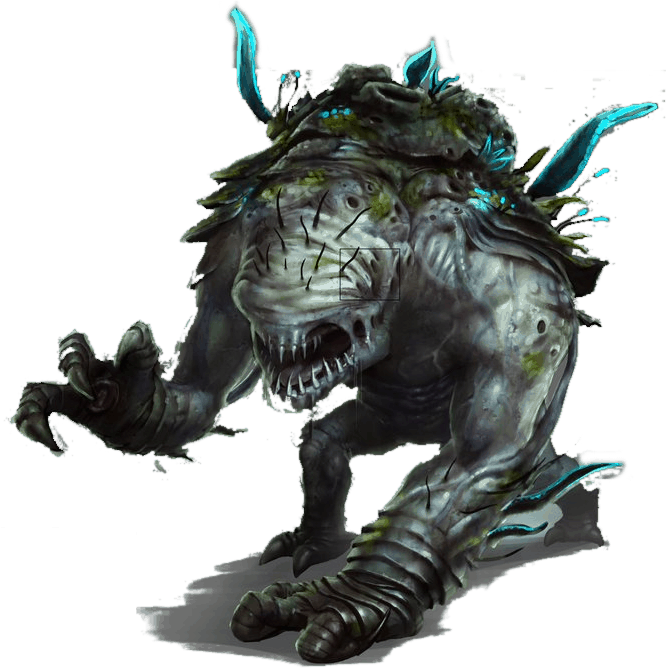
\includegraphics[width=\linewidth]{_img/dos-au-muur/rakghoul-amblyope.png}

Situé au pont inférieur, deuxième hangar. C’est l’étape finale et le boss de fin du scénario.

Le droïde ou un passage au poste de commande déverrouille la porte du hangar. \'A l’intérieur c’est une autre histoire, une créature de 2m de haut manifestement un rakghoul aux stéroïdes, un rakghoul Amblyope~\ref{sec:rakghoul-amblyope} p. \pageref{sec:rakghoul-amblyope}).

Selon vos héros et leur état, accompagnez le joker avec quelques rakghouls en extra. Les héros avec Sens de Force ressentent une forte présence du côté obscur autour de la créature.\\

Une fois le combat terminé, il ne leur reste plus qu’à prendre le vaisseau (Cargo léger YZ-775, le \nameref{sec:nimbus}). Ouf, les clefs sont sur le contact. L’armement du vaisseau est endommagé et ne fonctionne pas mais le reste est intact.

\subsection{To be continue\ldots}
Une fois en vol, vos héros reçoivent une communication d’origine inconnue, le visage d’une femme apparaît

\begin{quotebox}
	Tinon \emph{(prononcer Taïnon)} c’est toi ? Que se passe t’il ou va tu ?
\end{quotebox}

Rideau, suite au prochain épisode\ldots

\subsection{Progression}
A titre indicatif car c’est a vous de voir ce que vos héros méritent.

\begin{rebelist}
	\item \textbf{1xp} Si vos héros ont R4-3D avec eux à la fin du scénar.
	\item \textbf{1xp} Pour avoir tué le \nameref{sec:rakghoul-amblyope}.
	\item \textbf{1xp} Pour être sortie du vaisseau en vie.
\end{rebelist}
Pas plus de 3xp, le scénar n’est pas assez long pour mériter plus.

\clearpage
\subsection{Pelican (iA-1701)} \label{sec:pelican}
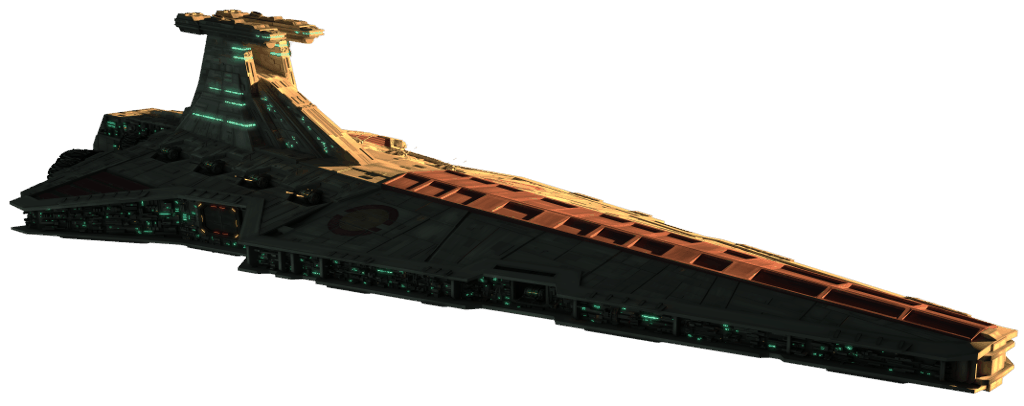
\includegraphics[width=\textwidth]{_img/dos-au-muur/venator.png}
\vspace{-4\baselineskip}

Quelques informations sur le Pelican. Il s’agit d’un croiseur de classe \textbf{Venator}. 1 137 m de long, 7400 hommes d’équipage, capable d’hyper-propulsion.

Le Pelican appartient à Industrial Automaton qui s’en sert comme vaisseau scientifique ultra-sécurisé. Ils y hébergent des projets top secret et aux limites de la loi.

\subsubsection{Journal de bord}
\label{sec:pelican-jdb}
En relation étroite avec l’Empire, Industrial Automation envoie le Pelican à la recherche d’un ancien artefact Sith, le Talisman de Muur. Le Pelican a fini par trouver une trace du Talisman sur \href{http://fr.starwars.wikia.com/wiki/Taris}{Taris}. En fouillant les bas fonds de la planète, l’équipe de chercheurs trouve les vestiges d'un ancien temple Sith. Malheureusement ce dernier est infesté de Rakghouls. L’unité de sécurité qui accompagne les chercheurs parvient à se débarrasser des quelques créatures mais plusieurs hommes sont blessés pendant le combat. Dans les ruines du temple le Talisman n’est plus là, mais des indices tendent à penser qu’il a été transporté il y a très longtemps vers une planète éloignée mais les scientifiques n’ont pas eu le temps d’en apprendre plus. Ils décident alors de ramener les corps des Rakghouls à bord du Pelican et de retourner sur Gaulus, une planète rocailleuse aux confins de la bordure extérieure.

En chemin vers Gaulus les scientifiques étudient le corps du Rakghoul et apprennent qu’il s’agit d’une maladie qui semble artificielle. La maladie se transmet par griffure ou morsure. Cette maladie est étroitement liée au côté Obscur de la Force et il semble que les personnes sensibles à la force ne puissent être contaminées. Cependant le Rakghoul étudié a l’air d’être contaminé par une forme très basique du virus, certainement une exposition prolongée à l’artefact.

Après une semaine de voyage, les problèmes ont commencé. Les soldats blessés lors de la rixe contre les Rakghouls sur Taris commencent à se transformer en Rakghouls à leur tour et s’en prennent aux membres de l’équipage. C’est une boucherie sans nom ! Voyant cela, le commandant du Pelican (\emph{Tycho Obrin}) déclenche le protocole d’urgence consistant à enregistrer le journal de bord sur un droïde Type R et tente de bloquer le cap du vaisseau sur l’étoile la plus proche. Mais la propulsion est endommagée et bien que le cap du vaisseau soit bloqué, ce dernier se contente de dériver.

\vspace{10\baselineskip}
\subsubsection{Industrial Automaton}
N’ayant plus de nouvelle du Pelican depuis son départ de Taris, IA part à sa recherche. Ils le retrouvent et envoient une équipe à son bord, mais là encore, plus aucune nouvelles. C’est alors qu’IA décide d’envoyer des mercenaires. Si le commandant a respecté le protocole, il suffira que les mercenaires ramènent le droïde\ldots

\onecolumn
\subsubsection{Plan du vaisseau}

\begin{figure}[!h]
	\centering
	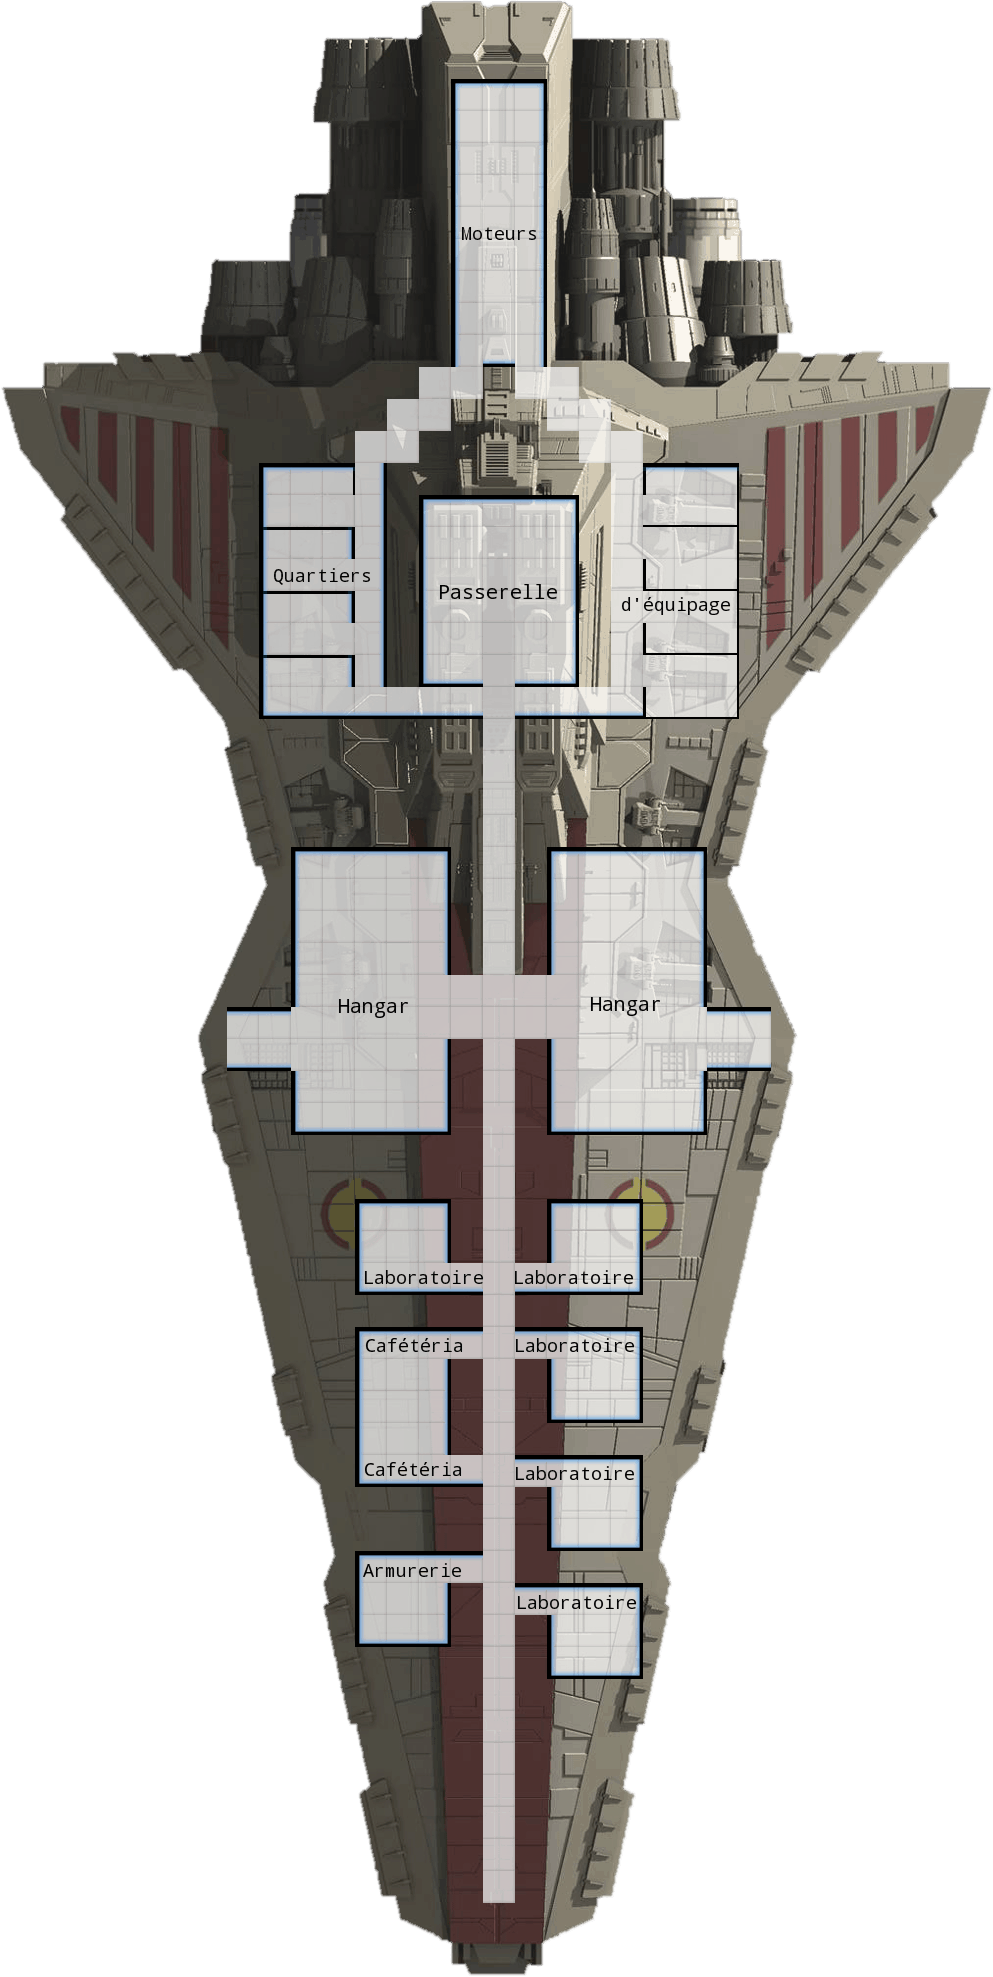
\includegraphics[height=0.87\textheight]{_img/dos-au-muur/venator-plan.png}
	\caption{Ce n’est qu’une proposition, le plan peut changer à volonté. En annexe, vous trouverez des cases permettant de faire découvrir le vaisseau petit à petit aux héros.}
\end{figure}

\twocolumn
